\section{OLD STUFF: Localization with LoRa}
\label{sec:old-localization}
% {\color{blue} [SWARUN, DIANA]}

% what we do / motivation
% In this section, we detail our approach to build a framework for  inexpensive, LP-WAN radios to localized both indoors and outdoors using commodity base station infrastructure. Doing so would allow a range of applications where people, pets and common objects can be tracked using inexpensive tags powered by 10-year batteries, whether indoors or outdoors. Such tags can be affixed to mail, packages and goods as they are sent from source to destination, to visualize their current position in real time and track them down in case they are lost. One can also imagine smart fabrics equipped with these tags used to track the location of persons who may otherwise not carry GPS-enabled smart devices such as children, the elderly, or physically challenged.   

%  past work


% The proposed work...
In this section, we detail our approach to build a framework for localization of inexpensive, LP-WAN radios both indoors and outdoors using commodity base station infrastructure. We do this using a mechanism that ensures client devices remain low-power and low-cost, while delegating software-only processing of signal information at the base stations. 
%Our approach allows a range of applications where people, pets and common objects can be tracked using inexpensive tags powered by 10-year batteries, whether indoors or outdoors. It also forms a critical piece of our location-aware network management framework for LP-WANs, aiding whitespace database lookup and enabling deployment of a live heatmap of radio performance measured over large urban spaces. 

% Define the primitive
Our localization solution relies on a simple primitive -- a mechanism that allows pairs of LP-WAN client devices to estimate their pair-wise distances at meter-level accuracy. We do this by accurately estimating time-of-flight between any two radios. The time-of-flight, when multiplied by the speed of light can be used to compute the distance between two devices. By computing the distance between pairs of adjacent devices, whether client or base station, one can obtain a series of geometric relationships between different radios at different geographic locations. We can then use this information to infer the location of client devices, given the known locations of the base stations and/or certain clients.  

% Challenges in building the primitive
Yet, building the above pairwise localization primitive has several challenges: (1) {\it Obtaining  time-of-flight from wireless channels: } To measure time-of-flight accurately, one would need to measure wireless channel state information on low-power platforms across wide bandwidth. However, many LP-WAN protocols (\emph{e.g.,} SigFox and NB-IoT) are narrow band owing to power constraints, leading to several hundred meters of positioning error. More crucially, they employ simple receivers that are not designed to obtain wireless channel state information. (2)  {\it Hardware Non-Idealities: } The low-power nature of client devices would mean any channels gathered are subject to timing errors, phase shifts and frequency offsets, that must be eliminated. (3) {\it Finding Absolute Location: } While our primitive obtains pair-wise distances, one would need a mechanism to obtain the absolute location of client devices. We aim to do so without requiring all client devices to be in radio range of more than one base station -- a common scenario in the LP-WAN context. Next, we describe our solution to each of the above challenges.  
%using simple hardware and software modifications at client devices and base station. 

% Diana's text
% Current localization technologies are specialized for either indoor or outdoor use. Indoor localization technologies rely on fixed beacons which do not move in a typical residential or commercial building, such as a WiFi router. These beacons also typically have a limited range. Outdoor localization typically uses GPS, which is both power-hungry and attenuated by walls. For applications that require both indoor and outdoor localization, such as tracking pets, children, and packages, the current state-of-the-art is insufficient.

% Furthermore, urban environments are, by their nature, dense with obstacles and competing devices. In such circumstances, it can be difficult for a node to transmit to a single beacon, much less to three (as is required for trilateration). This could be solved with a higher transmit power, which would shorten the battery lifespan of these devices, or increasing the density of the beacons in urban environments, which is both time-consuming and expensive.

% Thus, we propose our system, which uses pairwise localization and previously out-of-range access points to determine positions of its constituent nodes.

\subsection{Computing time-of-flight}
Our first challenge is to measure time of flight between pairs of low-power wireless radios. Traditionally, measuring time-of-flight requires radios that span a wide bandwidth. Yet, LP-WAN radios are intrinsically designed to be narrow-band owing to their low power requirements  -- a few hundred kilohertz at best. This vastly limits its resolution in  time-of-flight to hundreds of meters at best. 

\begin{figure*}[!htb]
\centering
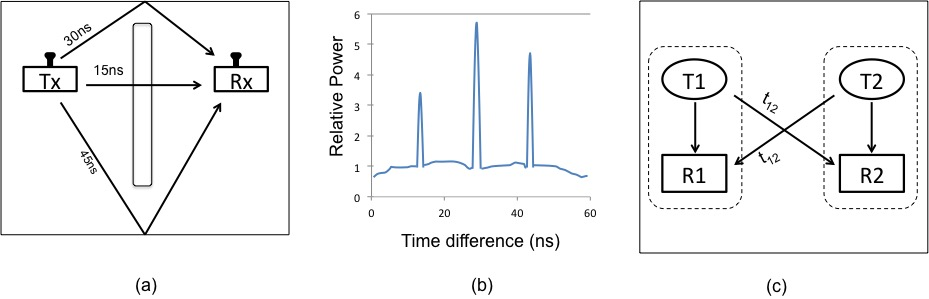
\includegraphics[width=0.9\textwidth]{figures/experiment.jpg}
\compactimg
\caption{(a) Depicts the wireless signal from a transmitter to receiver traversing there signal paths. (b) A plot of the relative signal power received corresponding to different times-of-flight. The first peak corresponds to the direct signal path. (c) Our localization framework leverages channel measurements at receivers that are co-located with the two LP-WAN clients to measure the relative time-of-flight between them: $t_{12}$.}
\label{fig:localize}
\end{figure*}

Our solution to overcome this challenge exploits the fact that LP-WAN radios, while being narrowband, regularly hop between a wide range of frequencies due to FCC mandated frequency-hopping. Our key idea is to stitch together wireless channel state information (CSI) measurements from these open frequencies to emulate a wide-band radio. Indeed, LP-WAN radios have a range of available frequencies to operate on -- including the 433~MHz, 900~MHz and whitespace frequencies (several bands in the 450-700 MHz range), together spanning a very wide bandwidth. Channel State Information obtained from these frequencies can then be processed to obtain time of flight at  a significantly higher resolution -- a few meters. Our solution builds upon recent work to combine channel information across frequencies in the WiFi context~\cite{vasisht2016decimeter}, while accounting for properties unique to LP-WANs such as power-constraints, hardware imperfections and limited receive-capability of LP-WAN hardware. 

To demonstrate our approach, mathematically, consider a signal that experiences a time-of-flight $\tau_{12}$ when traversing from a transmitter-1 to receiver-2 along line-of-sight. We assume that the transmitter and receiver operate on identical frequencies and are synchronized in time and phase (we consider hardware non-idealities in Sec.~\ref{sec:nonideal}). We can write the wireless channel experienced by this signal at any frequency $f$ as:
\begin{align}
h_f = A e^{-j 2 \pi f \tau_{12}}
\end{align}

where $A$ is signal the amplitude. %The phase of the channel is thus:
%
%\begin{align}
%\angle h_f = -j 2 \pi f %\tau_{12}~~\mod 2\pi %\label{eqn:channelphase}
%\end{align}
%
Solving for $\tau_{12}$, we find
%
\begin{align}
\tau_{12} = -\angle h_f /{(2 \pi f)}~~~\mod	1/f	\label{eqn:channelphase}
\end{align}
%
Note that the above equation computes time-of-flight modulo $1/f$. By hopping across a range of frequencies, one would obtain the time-of-flight with different modulo values. By combining these equations (using the Chinese Remainder Theorem~\cite{vasisht2016decimeter, ding1996chinese}), one can compute the time-of-flight with high resolution. We note that the above approach can be readily extended to settings where signals traverse more than one path, by combining measurements across frequencies.  Here, one can apply standard signal processing algorithms such as Bartlett~\cite{kumar2014accurate} or MUSIC~\cite{xiong2013arraytrack} to estimate the power of the signals along paths corresponding to different times-of-flight:
\begin{align}
P(\tau) = \left|\sum_f h_f e^{2 \pi f \tau}\right|^2 \label{eqn:ptau}
\end{align}
Fig.~\ref{fig:localize}(b) depicts this profile computed for a simple example of signals traversing along three paths as shown in Fig.~\ref{fig:localize}(a). Of the three paths, the direct path is the shortest and corresponds to the least time-of-flight. Hence, we can compute distance between the two devices by simply identifying the first peak in $P(\tau)$.

We note that the above approach requires measuring wireless channel state information on client devices. However, building a low-energy mechanism to do so on commodity LP-WAN devices is challenging. Indeed commodity radios from LoRa and SIGFOX are employ simple receive chains that are not designed to provide low-level signal information~\cite{alliance2015lorawan, zuniga2016sigfox}.

%\bob{SigFox implements a downlink, and it is described in the referenced IETF document.  Network practices severely limit the number of daily downlink messages per day (four).  Weightless-N was originally a one-way scheme.  Weightless-P tries to fix that.  The real limitation on Class A LoRa downlink messages is that they have to be queued and are dependent on the device initiating a transmit-receive sequence.} 

To resolve this challenge, we advocate augmenting some LP-WAN clients that have available wall-power, with low-cost receivers that are capable of obtaining channel state information. These radios can then be co-located with a subset of transmitting devices and record wireless channels from the base station and nearby devices. Given that these devices need to only measure CSI and not perform full-scale decoding, we can implement them using cheap off-the-shelf hardware. Our proof-of-concept implementation in Sec.~\ref{sec:eval} considers a subset of LP-WAN clients equipped with low-cost ($\sim$ \$10) RTL-SDR software radios~\cite{rtlsdr}.\footnote{We believe future designs can incorporate low-power CC1200 radios that provide channel state information, while drawing only 0.5$\mu$A of current when idle.} In this scenario, one must still  localize battery-powered client devices that do not have sophisticated receive chains -- a challenge we overcome in Sec.~\ref{sec:localization-inter}.

 

\subsection{Hardware Non-Idealities}\label{sec:nonideal}

Our discussion thus far has ignored a critical challenge faced by low-cost transmitters and receivers -- their hardware non-idealities. Specifically, low-power radios are driven by inexpensive oscillators that tend to drift over time. This drift creates three different offsets in the channel state-information gathered between low-power client devices: (1) A Frequency Offset: Stemming from the fact that the transmitter and receiver may operate at slightly different center frequencies; (2) A Timing Offset: The receiver may detect the transmitted signal at an arbitrary delay, which affects the measured channel state information; (3) A Phase Offset: A random phase error introduced to the CSI whenever the hardware restarts, introduced by the Phase Locked Loop (PLL) of the transmitter and receiver. 

Mathematically, these three offsets have a direct impact on the phase of the wireless channel. In particular, we can re-write Eqn.~\ref{eqn:channelphase} of the wireless channel captured at time $t$ to incorporate offsets in time $\Delta t$, frequency $\Delta f$ and phase $\Delta \phi$ as follows:
\begin{align}
\angle h_f = -j~(2 \pi f \tau_{12} + 2 \pi \Delta f t + 2 \pi f \Delta \tau + \Delta \phi) ~~\mod 2\pi
\end{align}

Complicating matters further is the fact that our nodes have two radios each -- one to transmit and one to receive channel state information, each driven by different clocks. This implies that we get four unique values for each offset, one between every transmitter-receiver pair within and across client nodes.

We overcome this challenge by exploiting the structure of  frequency offsets. Specifically, we leverage the fact that given that transmitters and receivers are co-located, their relative time-of-flight is known a priori. As a result, one can use estimates of the channel between the co-located transmitter-receiver pair at each client node to remove the offsets between two nodes. 

To illustrate our approach mathematically, let's consider the configuration shown in Fig.~\ref{fig:localize}(c).  Here, the sender $T_1$ with time delay $\Delta t_1$, frequency $f_1$, phase $\phi_1$, transmits a signal received with time delay $\Delta t_2$, frequency $f_2$, phase $\phi_2$ by $R_2$. We can then write the wireless channel between transmitter $T_1$ and receiver $R_2$ as:
\begin{align}
\angle h_{T_1 \rightarrow R_2} = -j~(2 \pi f_{R_2} \tau_{12} + 2 \pi (f_{T_1} - f_{R_2}) t\hspace*{2cm} \nonumber \\
+ 2 \pi f (\Delta t_{T_1} + \Delta t_{R_2}) +(\phi_{T_1} - \phi_{R_2}) ) ~~\mod 2\pi \label{eqn:h1}
\end{align}
One can then write similar equations for channels between every transmitter, receiver pair. However,  note two properties: First, the time-of-flight and delays between co-located transmitter, receiver pairs is constant -- and can therefore be calibrated a-priori. Without loss of generality, we can assume the time-of-flight is zero to write:
\begin{align}
\angle h_{T_1 \rightarrow R_1} = -j~(2 \pi (f_{T_1} - f_{R_1}) t + 2 \pi f (\Delta t_{T_1} + \Delta t_{R_1})  \nonumber \\
+~(\phi_{T_1} - \phi_{R_1}) ) ~~\mod 2\pi \label{eqn:h22}
\end{align}
Second, the time-of-flight experienced by signals from the transmitter to receiver and vice-versa are identical. 
%In other words, we can write the channels from $T_2$ to $R_1$ as:
%\begin{align}
%\angle h_{T_2 \rightarrow R_1} =&  -j~(2 \pi f_{R_1} \tau_{12} + 2 \pi (f_{T_2} - f_{R_1}) t   \nonumber \\
%& + 2 \pi f (\Delta t_{T_2} + \Delta t_{R_1}) +~(\phi_{T_2} - \phi_{R_1}) ) ~~\mod 2\pi \label{eqn:h3}
%\end{align}
Combining Eqn.\ref{eqn:h1}-\ref{eqn:h22}:
\begin{align}
\angle \left(\frac{h_{T_1 \rightarrow R_2} h_{T_2 \rightarrow R_1}}{h_{T_1 \rightarrow R_1} h_{T_2 \rightarrow R_2}} \right) = -j~4 \pi f_{R_1} \tau_{12} ~~\mod 2\pi \label{eqn:h4}
\end{align}
Therefore,  $\hat{h}_f = \frac{h_{T_1 \rightarrow R_2} h_{T_2 \rightarrow R_1}}{h_{T_1 \rightarrow R_1} h_{T_2 \rightarrow R_2}}$ is independent of frequency offsets. Hence, we can rewrite Eqn.~\ref{eqn:ptau} using the modified channels, to measure time-of-flight in the presence of multiple signal paths as:
\begin{align}
P(\tau) = \left|\sum_f \frac{h_{T_1 \rightarrow R_2} h_{T_2 \rightarrow R_1}}{h_{T_1 \rightarrow R_1} h_{T_2 \rightarrow R_2}} e^{4 \pi f \tau}\right|^2 =  \left|\sum_f \hat{h}_f e^{4 \pi f \tau}\right|^2\label{eqn:ptau2}
\end{align}

Thus, we can estimate time-of-flight between two clients, despite the two radios on each experiencing arbitrary hardware offsets. 


\subsection{Finding Absolute Localization}\label{sec:localization-abs}
Given relative locations as calculated from pairwise times-of-flight, one would still need to find the absolute location of client nodes. We must do so solely using given pairwise distances between several pairs of nodes -- some of which at known absolute locations (e.g. the base stations themselves). However, our approach should also deal with uncertainty in observed distances, owing to  noise. 

We propose to exploit the extensive past work on network localization to overcome this problem. Past work has shown how one can model the wireless network topology as a graph with pair-wise distances between sensor nodes along with their uncertainties labeled as edge weights~\cite{nwlocalization}. Assuming that the graph is rigid, one can then use the known location of a subset of these nodes to calculate the location of the remaining nodes~\cite{sethnwlocalization}.


\subsection{Locating Battery-Powered Devices and Sources of Interference}\label{sec:localization-inter}

This section extends our localization framework to devices where channel state information is not available. For instance, consider battery-powered LP-WAN nodes whose RF-chains are not sophisticated enough to measure channel state information. Or consider interferers transmitting on the same frequencies, whose channel state information is not available to the network. Our approach to locate these devices leverages the availability of nearby powered clients that can measure signals from these nodes. However, a crucial challenge when dealing with interfering sources, in particular, is that their channels cannot also be measured at our own powered clients, given that the signals interferers transmit are potentially unknown. In other words, we would need to locate  interferers without knowledge of their transmitted signals or any cooperation. 

We address this challenge by measuring time-difference of arrival, as opposed to time-of-arrival between a transmitting source and two powered clients that listen to the node of interest. Specifically, for each transmitter $I$, we capture the wireless signal $y_{I->R_1}$ and $y_{I->R_2}$ measured by the receive chains of our two clients. One can then write these received signal as a function of the potentially unknown transmitted signal $x_I$, and  corresponding channels as: 
\begin{align*}
y_{I->R_1} =  h_{I->R_1} x_I \text{~~and~~} y_{I->R_2} = h_{I->R_2} x_I 
\end{align*}

It is then easy to see that $y_{I->R_1}/y_{I->R_1}$ is a function independent of the transmitted signal and depends purely on the wireless channels from the transmitter to the receive chains. More specifically, it depends on the time-difference of arrival between the transmitter to either receiver. However, like before, it is once again subject to time, frequency and phase offsets. Interestingly, the time-difference of arrival can be written purely in terms of the hardware non-idealities of our own powered clients. To see how, observe that: 
\begin{align*}
\angle y_{I \rightarrow R_1} /  y_{I \rightarrow R_2} = & -j~(2 \pi f_{R_2} (\tau_{I \rightarrow R_1} - \tau_{I \rightarrow R_2}) + 2 \pi (f_{R_1} - f_{R_2}) t \nonumber \\
& + 2 \pi f_{R_2} (\Delta t_{R_1} - \Delta t_{R_2})  +~(\phi_{R_1} - \phi_{R_2}) ) \mod 2\pi \label{eqn:h2}
\end{align*}

Let's assume that at the same time $t$ we have a packet sent from one of the transmit chains of our powered clients to the two receivers, we can then write:
\begin{align*}
\angle h_{T_1 \rightarrow R_1} /  h_{T_1 \rightarrow R_2} = & -j~(- 2 \pi f_{R_2}\tau_{12} + 2 \pi (f_{R_1} - f_{R_2}) t \nonumber \\
& + 2 \pi f_{R_2} (\Delta t_{R_1} - \Delta t_{R_2})  +~(\phi_{R_1} - \phi_{R_2}) ) \mod 2\pi 
\end{align*}

Combining the above two equations, we observe that the quantity $\frac{y_{I \rightarrow R_1} h_{T_1 \rightarrow R_2}}{y_{I \rightarrow R_2} h_{T_1 \rightarrow R_1}}$ is independent of hardware offset as well as the transmitted signal of $I$ and depends purely on the time-difference of arrival $\tau_{I \rightarrow R_1} - \tau_{I \rightarrow R_2}$, as well as the known time-of-flight $\tau_{12}$ between our two powered sensor clients. Consequently, we can measure the time-difference-of-arrival by extending Eqn.~\ref{eqn:ptau2} as:
\begin{align}
P(\tau) = \left|\sum_f \frac{y_{I \rightarrow R_1} h_{T_1 \rightarrow R_2}}{y_{I \rightarrow R_2} h_{T_1 \rightarrow R_1}} e^{4 \pi f (\tau + \tau_{12}) }\right|^2 
\end{align}
By computing the time-differences between  $I$ and three or more powered clients, one can obtain its location relative to them. Given that the absolute location of powered clients can be obtained using the algorithms in Sec.~\ref{sec:localization-abs}, one can obtain the absolute position of  interfering and battery-powered sources as well.
